
%ozeki??

\chapter{State of the Art}	\label{chap:sota}
This chapter presents an overview over the various published approaches for the tasks considered in this work. One key issue is comparability: As in many MIR tasks, data sets are not publicly available and vary widely, which makes  comparison of the individual approaches very difficult. As the following sections show, there is also disagreement about evaluation measures in all of these tasks.\\

For these reasons, new, reproducible data sets were created for this work (presented in the next chapter). As described in the previous chapter, the most frequently used measures were employed for evaluation.

\section{From speech to singing} \label{sec:sota_speechtosinging}
Singing presents a number of challenges for speech recognition when compared to pure speech \cite{loscos}\cite{goto_alignment}\cite{kruspe_kws1}. The following factors make speech recognition on singing more difficult than on speech, and necessitate the adaption of existing algorithms.
\begin{description}
 \item[Larger pitch fluctuations] A singing voice varies its pitch to a much higher degree than a speaking voice. It often also has very different spectral properties.
 \item[Larger changes in loudness] In addition to pitch, loudness also fluctuates much more in singing than in speech.
 \item[Higher pronunciation variation] The musical context causes singers to pronounce certain sounds and words differently than if they were speaking them.
 \item[Larger time variations] In singing, sounds are often prolonged for a certain amount of time to fit them to the music. Conversely, they can also be shortened or left out completely.
 In order to research this effect more closely, a small experiment was performed on a speech corpus and on a singing data set (\textit{TIMIT} and \textit{ACAP}, see chapter \ref{chap:datasets}): The standard deviations for all the phonemes in each data set were calculated. The result is shown in figure \ref{fig:phoneme_stats}, confirming that the variation in singing is much higher. This is particularly true for vowels.
 \item[Different vocabulary] In musical lyrics, words and phrases often differ from normal conversational script. Certain words and phrases have different probabilities of occurring in speech versus singing (e.g. a higher focus on emotional topics in singing).
 \item[Background music] This is the biggest interfering factor with polyphonic recordings. Harmonic and percussive instruments add a big amount of spectral components to the signal, which lead to confusion in speech recognition algorithms. Ideally, these components should be removed or suppressed in a precursory step. This could be achieved, for example, by employing source separation algorithms, but such algorithms add additional artifacts to the signal, and may not even be sufficient for this purpose at the current state of research.
 Vocal Activity Detection (VAD) could be used as a non-invasive first step in order to discard segments of songs that do not contain singing voices. However, such algorithms often make mistakes in the same cases that are problematic for speech recognition algorithms (e.g. instrumental solos \cite{schlueter2016_ismir}).
 For these reasons, most of the experiments in this work were performed on unaccompanied singing. The integration of the mentioned pre-processing algorithms would be a very interesting next step of research.
The lyrics-to-singing alignment algorithms presented in chapter \ref{chap:retrieval_alignment} are an exception. Those were also tested on polyphonic music, and the algorithms appear to be largely robust to these influences.
 \end{description}
 
 %Mehr Beispiele aus Goto-Kapitel
 %Sundberg!
 % Vowels vs. Consonants (1. Mesaros-Paper + recognition of phonemes and words...)

\begin{figure*}
	\begin{center}
		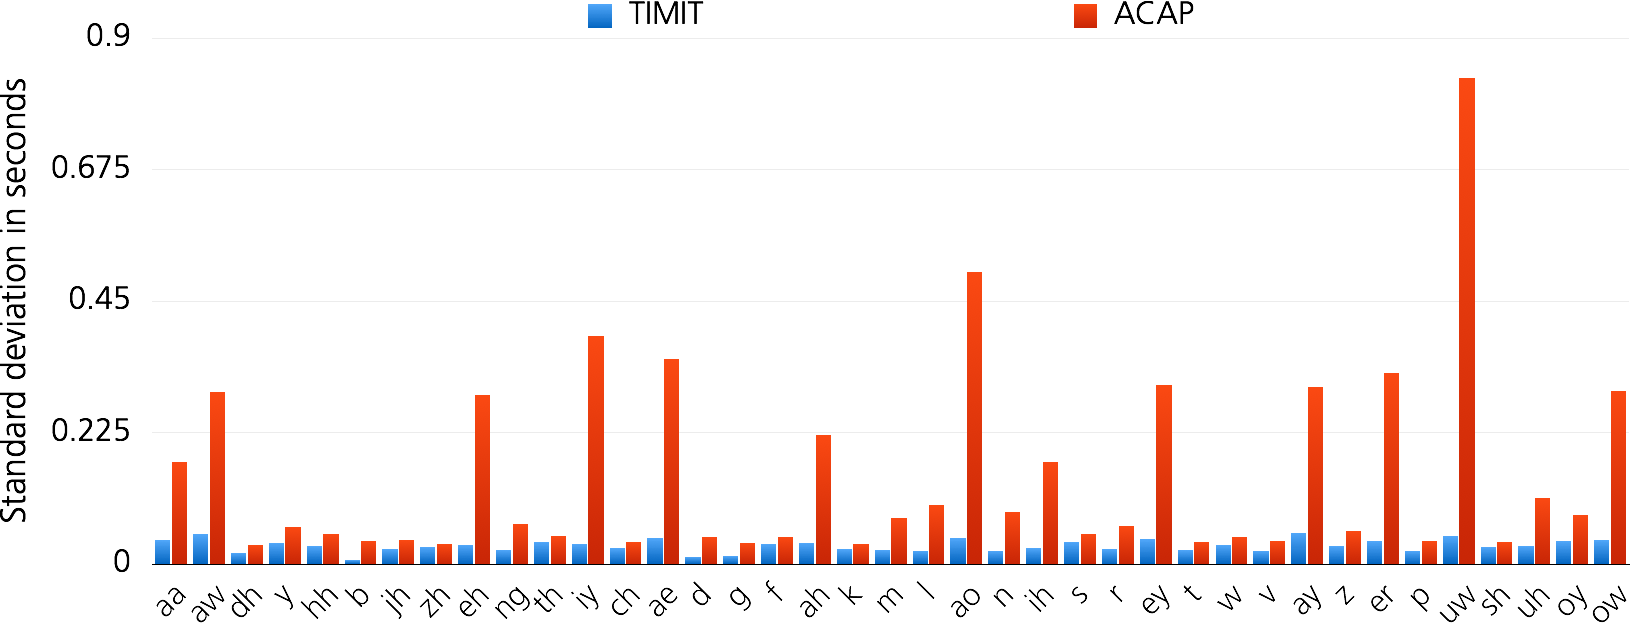
\includegraphics[width=1\textwidth]{images/phoneme_stats.png}
		\caption{Standard deviations of phoneme durations in the \textit{TIMIT} and \textit{ACAP} data sets.}
		\label{fig:phoneme_stats}
	\end{center}
\end{figure*}

The broad field of analyzing various aspects of the singing voice was summed up as \textit{singing information processing} in \cite{singing_information_processing} (updated in \cite{singing_information_processing2}). A first collection of singing voice recordings for Music Information Retrieval was created in 2005 \cite{jap_humming} (this database is not used in this work because it is not publicly available).

%describe tasks here??

\section{Phoneme recognition} \label{sec:sota_phonerec}
%\subsection{Phoneme recognition in speech}
%\subsection{Phoneme recognition in singing}
Due to the factors mentioned above in section \ref{sec:sota_speechtosinging}, phoneme recognition on singing is more difficult than on clean speech. It has only been a topic of research for a few years, and there are few publications.\\

One of the earliest systems was presented by Wang et al. in 2003 \cite{WangLC03}. Acoustic modeling is performed with triphone HMMs trained on read speech in Taiwanese and Mandarin. The language model is completely restricted to lines of lyrics in the test dataset. Testing is performed on 925 unaccompanied sung phrases in these language. Due to the highly specific language model, the Word Error Rate is just $0.07$.\\

Hosoya et al. employ a similarly classic approach from ASR that employs monophone HMMs also trained on read speech for acoustic modeling \cite{Hosoya2005} (2005). These models are adapted to singing voices using the Maximum Likelihood Linear Regression (MLLR) technique \cite{mllr}. Language modeling is performed with a Finite State Automaton (FSA) specific to the Japanese language, making it more flexible than the previous system.
The system is tested on five-word unaccompanied phrases, while the adaptation is performed on 127 choruses performed by different singers. The Word Error Rate is $0.36$ without the adaptation, and $0.27$ after adaptation.\\

In 2007, Gruhne et al. presented a classic approach that employs feature extraction and various machine learning algorithms to classify singing into 15 phoneme classes \cite{Gruhne2007} \cite{Gruhne2007a}. The specialty of this approach lies in the pre-processing: At first, fundamental frequency estimation is performed on the audio input, using a Multi-Resolution Fast Fourier Transform (MRFFT) \cite{inproceedings:dressler}. Based on the estimated fundamental frequency, the harmonic partials are retrieved from the spectrogram. Then, a sinusoidal re-synthesis is performed, using only the detected fundamental frequency and partials. Feature extraction is then performed on this re-synthesis instead of the original audio. Extracted features include MFCCs, PLPs, Linear Predictive Coding features (LPCs), and Warped Linear Predictive Coding features (WLPCs \cite{lpc}). MLP, GMM, and SVM models are trained on the resulting feature vectors. The re-synthesis idea comes from a singer identification approach by Fujihara \cite{fujihara_identification}. The approach is tested on more than 2000 separate, manually annotated phoneme instances from polyphonic recordings. Only one feature vector per phoneme instance is calculated. Using SVM models, $56\%$ of the tested instances were classified correctly into one of the 15 classes. This is considerably better than the best result without the re-synthesis step ($34\%$). In \cite{szepannek} (2010), the approach is expanded by testing a larger set of perceptually motivated features, and more classifiers. No significant improvements are found when using more intricate features, and the best-performing classifier remains an SVM.\\

Fujihara et al. described an approach based on spectral analysis in 2009 \cite{fujihara_phonemes}. The underlying idea is that spectra of polyphonic music can be viewed as the weighted sum of two types of spectra: One for the singing voice, and one for the background music. This approach then models these two spectra as probabilistic spectral templates. The singing voice is modeled by multiplying a vocal envelope template, which represents the spectral structure of the singing voice, with a harmonic filter, which represents the harmonic structure of the produced sound itself. This is analogous to the source-filter model of speech production \cite{Fant1981}. For recognizing vowels, five such harmonic filters are prepared (\texttt{a - e - i - o - u}). Vocal envelope templates are trained on voice-only recordings, separated by gender. Templates for background music are trained on instrumental tracks. In order to recognize vowels, the probabilities for each of the five harmonic templates are estimated. 
As described, the phoneme models are gender-specific and only model five vowels, but also work for singing with instrumental accompaniment. The approach is tested on 10 Japanese-language songs. The best result is $65\%$ correctly classified frames, compared to the $56\%$ with the previous approach by this team, based on GMMs.\\

%As a side product, the algorithm also estimates the fundamental frequency of the singing voice
In these experiments, the fundamental frequencies $F_0$ (which are necessary for the recognition) are manually provided. The approach is further expanded in \cite{concurrent_f0_phonemes} to be able to detect them concurrently with the phonemes. Additionally, models can directly be trained on polyphonic music rather than monophonic singing voices. The over-all best results degrade by around 4 percent points, but this makes the method much more flexible.\\

In 2009, Mesaros et al. also picked Hosoya's approach back up by using MFCC features and GMM-HMMs for acoustic modeling \cite{Mesaros2009}, and adapting the models for singing voices. These models are trained on the CMU ARCTIC speech corpus\footnote{\url{http://festvox.org/cmu_arctic/}}. Then, different MLLR techniques for adapting the models to singing voices are tested \cite{mllr}.
The adaptation and test corpus consists of 49 voice-only fragments from 12 pop songs with durations between 20 and 30 seconds. The best results are achieved when both the means and variances of the Gaussians are transformed with MLLR. The results improved slightly when not just a single transform was used for all phonemes, but when they were grouped into base classes beforehand, each receiving individual transformation parameters. The best result is around $0.79$ Phoneme Error Rate on the test set.\\

In \cite{Mesaros2010} and \cite{Mesaros2011}, language modeling is added to the presented approach. Phoneme-level language models are trained on the CMU ARCTIC corpus as unigrams, bigrams, and trigrams, while word-level bigram and trigram models are trained on actual song lyrics in order to match the application case. The output from the acoustic models is then refined using these language models. The approach is tested on the clean singing corpus mentioned above, and on 100 manually selected fragments of 17 polyphonic pop songs. To facilitate recognition on polyphonic music, a vocal separation algorithm is introduced \cite{virtanen_separation}.
Using phoneme-level language modeling, the Phoneme Error Rate on clean singing is reduced to $0.7$. On polyphonic music, it is $0.81$. For the word recognition approach, the word error rate is $0.88$ on clean singing, and $0.94$ on the polyphonic tracks.\\

A more detailed voice adaptation strategy is tested in \cite{mesaros2}. Instead of adapting the acoustic models with mixed-gender singing data, they are adapted gender-wise, or to specific singers. With the gender-specific adaptations, the average Phoneme Error Rate on clean singing is lowered to $0.81$ without language modeling, and $0.67$ with language modeling. Singer-specific adaptation does not improve the results, probably because of the very small amount of adaptation data in this case.\\
%mvcivar, hosoya

In \cite{McVicar2014} (2014), McVicar et al. build on a very similar baseline system, but also exploit repetitions of choruses to improve transcription accuracy. This has been done for other MIR tasks, such as chord recognition, beat tracking, and source separation. They propose three different strategies for combining individual results: Feature averaging, selection of the chorus instance with the highest likelihood, and combination using the Recogniser Output Voting Error Reduction (ROVER) algorithm \cite{rover}. They also employ three different language models, two of which were matched to the test songs (and therefore not representative for general application). 20 unaccompanied, English-language songs from the RWC database \cite{rwc} were used for testing; chorus sections were selected manually. The best-instance selection and the ROVER strategies improve results considerably; with the ROVER approach and a general-purpose language model, the Phoneme Error Rate is at $0.74$ (versus $0.76$ in the baseline experiment), while the Word Error Rate is improved from $0.97$ to $0.9$. Interestingly, cases with a low baseline result benefit the most from exploiting repetition information.\\

The final system was proposed by Hansen in 2012 \cite{jens}. It also employs a classic approach consisting of a feature extraction step and a model training step. Extracted features are MFCCs and TRAP features. Then, MLPs are trained separately on both feature sets. As mentioned in section \ref{subsec:tech_trap}, each feature models different properties of the considered phonemes: Short-term MFCCs are good at modeling the pitch-independent properties of stationary sounds, such as sonorants and fricatives. On the flip side, TRAP features are able to model temporal developments in the spectrum, forming better representations for sounds like plosives or affricates.
The results of both MLP classifiers are combined via a fusion classifier, also an MLP. Then, Viterbi decoding is performed on its output.
The approach is trained and tested on a data set of 13 vocal tracks of pop songs, which were manually annotated with a set of 27 phonemes. The combined system achieves a recall of $0.48$, compared to $0.45$ and $0.42$ for the individual MFCC and TRAP classifiers respectively. This confirms the assumption that the two features complement each other. The phoneme-wise results further corroborate this.\\

Various publications suggest that phoneme recognition is not a trivial task for human listeners either. Recognition rates are in the range of 70 to 90\% for native speakers, depending on factors such the signal quality and the type of phoneme \cite{weber_smits}\cite{meyer_waechter}. For singing, much lower rates are reported \cite{hollien}.


\section{Language identification}
A first approach for language identification in singing was proposed by Tsai and Wang in 2004 \cite{tsai_wang}. At its core, the algorithm is similar to Parallel Phone Recognition followed by Language Modeling (PPRLM). However, instead of full phoneme modeling, they employ an unsupervised clustering algorithm to the input feature data and tokenize the results to form language-specific codebooks (plus one for background music). Following this, the results from each codebook are run through matching language models to determine the likelihood that the segment was performed in this language. Prior to the whole process, Vocal Activity Detection is performed. This is done by training GMMs on segments of each language, and on non-vocal segments. MFCCs are used as features.
The approach is tested on 112 English- and Mandarin-language polyphonic songs each, with 32 of them being the same songs performed in both languages. A classification accuracy of $0.8$ is achieved on the non-overlapping songs. On the overlapping songs, the accuracy is only $0.7$, suggesting some influence of the musical material (as opposed to the actual language characteristics). Misclassifications occur more frequently on the English-language songs, possibly because of accents of Chinese singers performing in English, and because of louder background music.\\

A second, simpler approach was presented by Schwenninger et al. in 2006 \cite{schwenninger}. They also extract MFCC features, and then use these to directly train statistical models for each language. Three different pre-processing strategies are tested: Vocal Activity Detection, distortion reduction, and azimuth discrimination. Vocal Activity Detection (or vocal/non-vocal segmentation) is performed by thresholding the energy in high-frequency bands as an indicator for voice presence over 1-second windows. This leaves a relatively small amount of material per song. Distortion reduction is employed to discard strong drum and bass frames where the vocal spectrum is masked by using a Mel-scale approach. Finally, azimuth discrimination attempts to detect and isolate singing voices panned to the center of the stereo scene.
The approach is tested on three small data sets of speech, unaccompanied singing, and polyphonic music. Without pre-processing steps, the accuracy is $0.84$, $0.68$, and $0.64$ respectively, highlighting the increased difficulty of language identification on singing versus speech, and on polyphonic music versus pure vocals. On the polyphonic corpus, the pre-processing steps do not improve the result.\\

In 2011, Mehrabani and Hansen presented a full PPRLM approach for sung language identification. MFCC features are run through phoneme recognizers for Hindi, German, and Mandarin; then, the results are scored by individual language models for each considered language. In addition, a second system is employed which uses prosodic instead of phonetic tokenization. This is done by modeling pitch contours with Legendre polynomials, and then quantizing these vectors with previously trained GMMs. The results are then again used as inputs to language models.
The approach is trained and tested on a corpus containing 12 hours of unaccompanied singing and speech in Mandarin, Hindi, and Farsi. The average accuracy for singing is $0.78$ and $0.43$ for the phoneme- and prosody-based systems respectively, and $0.83$ for a combination of both.\\

Also in 2011, Chandrasekhar et al. presented a very interesting approach for language identification on music videos, analyzing both audio and video features \cite {chandrasekhar}. On the audio side, the spectrogram, volume, MFCCs, and perceptually motivated Stabilized Auditory Images (SAI) are used as inputs. One-vs-all SVMs are trained for each language. The approach is trained and tested on 25,000 music videos in 25 languages. Using audio features only, the accuracy is $0.45$; combined with video features, it rises to $0.48$. It is interesting to note that European languages achieve much lower accuracies than Asian and Arabic ones. English, French, German, Spanish and Italian rank below $0.4$, while languages like Nepali, Arabic, and Pashto achieve accuracies above $0.6$. It is possible that the language characteristics of European languages make them harder to discriminate (especially against each other) than others.

\section{Keyword spotting}
%\subsection{Keyword spotting in speech}
%Igor Sz? oke, Petr Schwarz, Pavel Matejka, Luk?as Bur-get, Martin Karafi? at, Michal Fapso, and Jan Cernock`y.Comparison of keyword spotting approaches for infor- mal continuous speech. In Interspeech, pages 633?636, 2005.
%\subsection{Keyword spotting in singing}
%SPEECH HERE
%pedro!!
Keyword spotting in singing was first attempted in 2008 by Fujihara et al. \cite{hyperlinking_lyrics}. Their method starts with a phoneme recognition step, which is once again based on the vocal re-synthesis method described in \cite{fujihara_identification}. MFCCs and power features are extracted from the re-synthesized singing and used as inputs to a phoneme model, similar to Gruhne's phoneme recognition approach mentioned above in section \ref{sec:sota_phonerec}.  Three phoneme models are compared: One trained on pure speech and adapted with a small set of singing recordings, one adapted with all recordings, and one trained directly on singing. Viterbi decoding is then performed using keyword-filler HMMs to detect candidate segments where keywords may occur. These segments are then re-scored through the filler HMM to verify the occurrence. When the textual lyrics for a song are known, the system offers the additional possibility to use lyrics-to-audio alignment instead.
The method is tested on 79 unaccompanied Japanese-language songs from the RWC database \cite{rwc} with keywords containing at least 10 phonemes. The Phoneme Error Rate is $0.73$ for the acoustic models trained on speech, $0.67$ for the adapted models, and $0.49$ for the models trained on singing (it should be mentioned that the same songs were used for training and testing, although a cross-validation experiment shows that the effect is negligible). The employed evaluation measure is ``link success rate'', describing the percentage of detected phrases that were linked correctly to other occurrences of the phrase in the data set. In that sense, it is a sort of accuracy measure. The link success rate for detecting the keywords is $0.3$. The authors show that the result depends highly on the number of phonemes in the considered keyword, with longer keywords being easier to detect.\\

Building on this approach, a system named \textit{LyricListPlayer} was developed by Nakano and Goto in 2016 \cite{lyriclistplayer}. In this case, however, keywords are exclusively detected using lyrics-to-audio alignment and a subsequent search on the textual lyrics (which need to be available in advance). Monophone HMM acoustic models for English and Japanese similar to the ones mentioned above are employed. Those models are trained on a relatively small number of songs from the RWC database \cite{rwc} using power-based and MFCC features. An interesting addition is the further processing of these alignments: Natural Language Processing (NLP) techniques for topic modeling are applied to the lyrics, allowing users to search for similar keywords or phrases.\\

In 2012, Mercado et al. presented an approach to keyword spotting in singing based on a different principle: DTW between a sung query and the requested phrase in the song recording. In particular, Statistical Sub-Sequence DTW is the algorithm employed for this purpose. MFCCs are used as feature inputs, then the costs of the warping paths are calculated from all possible starting points to obtain candidate segments, which are then further refined to find the most likely position.
The approach is tested on a set of vocal tracks of 19 pop songs (see section \ref{subsec:data_hansen}) as the references, and recordings of phrases sung by amateur singers as the queries, but no quantitative results are given. The disadvantage of this approach lies in the necessity for audio recordings of the key phrases, which need to have at least similar timing and pitch as the reference phrases.\\

Finally, Dzhambazov et al. developed a score-aided approach to keyword spotting in 2015 \cite{dzhambazov_ismir}. A user needs to select a keyword phrase and a single recording in which this phrase occurs. The keyword is then modeled acoustically by concatenating recordings of the constituent phonemes (so-called acoustic keyword spotting). Similar to Mercado's approach, Sub-Sequence DTW is performed between the acoustic template and all starting positions in the reference recording to obtain candidate segments. These segments are then refined by aligning the phonemes to the score in these positions to model their durations. This is implemented with Dynamic Bayesian Network HMMs. Then, Viterbi decoding is performed to re-score the candidate segments and obtain the best match.
The approach is tested on a small set of unaccompanied Turkish-language recordings of traditional Makam music. The Mean Average Precision (MAP) for the best match is $0.08$ for the DTW approach only, and $0.05$ for the combined approach. For the top-6 results, the MAP is $0.26$ and $0.38$ respectively.


\section{Lyrics-to-audio alignment}
%\subsection{Forced alignment in speech}
%\subsection{Forced alignment in singing}
%mesaros
%Three techniques for im- proving automatic synchronization between music and lyrics: Fricative detection, filler model, and novel feature vectors for vocal activity detection
In contrast to the other tasks discussed in this chapter, the task of lyrics-to-audio alignment has been the focus of many more publications. A comprehensive overview until 2012 is given in \cite{goto_alignment}.\\

A first approach was presented in 1999 by Loscos et al. \cite{loscos}. The standard forced alignment approach from speech recognition is adapted to singing. MFCCs are extracted first, and then a left-to-right HMM is employed to perform alignment via Viterbi decoding. Some modifications are made to the Viterbi algorithm to allow for low-delay alignment. The approach is trained and tested on a very small (22 minutes) database of unaccompanied singing, but no quantitative results are given.\\

The first attempt to synchronize lyrics to polyphonic recordings was made by Wang et al. in 2004 \cite{Wang2004}. They propose a system, named ``LyricAlly'', to provide line-level alignments for karaoke applications. Their approach is heavily based on musical structure analysis. First, the hierarchical rhythm structure of the song is estimated. The result is combined with an analysis of the chords and then used to split the song into sections by applying a chorus detection algorithm. Second, Vocal Activity Detection (VAD) using HMMs is performed on each section. Then, sections of the text lyrics are assigned to the detected sections (e.g. verses, choruses). In the next step, the algorithm determines whether the individual lines of the lyrics match up with the vocal sections detected by the VAD step. If they do not, grouping or partitioning is performed. This is based on the assumption that lyrics match up to rhythmic bars as determined by the hierarchical rhythm analysis. The expected duration of each section and line is estimated using Gaussian distributions of phoneme durations from a singing data set. In this manner, lines of text are aligned to the detected vocal segments. The approach is tested on 20 manually annotated pop songs. On the line level, the average error is $0.58$ seconds for the starting points and $-0.48$ seconds for the durations. The system components are analyzed in more detail in \cite{lyrically}.\\

In 2006, the same team presented an approach that also performs rhythm and bar analysis to facilitate syllable-level alignment \cite{Iskandar:2006}. For the phoneme recognition step, an acoustic model is trained on speech data and adapted to singing using the previously mentioned 20 songs. The possible syllable positions in the alignment step are constrained to the note segments detected in the rhythm analysis step. Due to annotator disagreement on the syllable level, the evaluation is performed on the word level. On three example songs, the average synchronization error rate is $0.19$ when allowing for a tolerance of 1/4 bar.\\  

Sasou et al. presented a signal parameter estimation method for singing employing an auto-regressive HMM (AR-HMM) in 2005 \cite{Sasou2005AnAN}. This method is particularly suited for modeling high-pitched signals, which is important for singing voices and usually not a focus in speech processing techniques. Models trained on speech are adapted to singing using MLLR. For evaluation, the method is applied to the task of lyrics-to-audio alignment and tested on 12 Japanese-language songs. For each song, a specific language model is prepared. The correct word rate is $0.79$.\\

Chen et al. presented an approach based on MFCC features and Viterbi alignment in 2006 \cite{popular_synchronization}. Vocal Activity Detection is performed as a pre-processing step, and then GMM-HMMs are used for Viterbi alignment between the audio and the lyrics. Once again, MLLR is used to adapt the acoustic models to singing. In addition, the grammar is specifically tailored to the lyrics. On a data set of Chinese songs by three singers, a boundary accuracy of $0.76$ is obtained on the syllable level.\\

A similar approach which does not require in-depth music analysis was presented by Fujihara et al. in 2006 \cite{fujihara_alignment}. Once again, a straightforward Viterbi alignment method from speech recognition is refined by introducing three singing-specific pre-processing steps: Accompaniment sound reduction, Vocal Activity Detection, and phoneme model adaptation.
For accompaniment reduction, the previously mentioned harmonic re-synthesis algorithm from \cite{fujihara_identification} is used. For Vocal Activity Detection, a HMM is trained on a small set of unaccompanied singing using LPC-derived MFCCs and fundamental frequency ($F_0$) differences as features. The HMM can be parameterized to control the rejection rate. For the phoneme model adaptation, three consecutive steps are tested: Adaptation to a clean singing voice, adaptation to a singing voice segregated with the accompaniment reduction method, and on-the-fly adaptation to a specific singer. MFCC features are used for the Viterbi alignment, which is performed on the vowels and syllabic nasals (\texttt{/m/, /n/, /l/}) only.
Ten Japanese pop songs were used for testing. Evaluation was done on the phrase level by calculating the proportion of the duration of correctly aligned sections to the total duration of the song. For eight of the ten songs, this proportion was $0.9$ or higher when using the complete system, which the authors judge as satisfactory. Generally, the results are lower for performances by female singers, possibly because of the higher $F_0$s. These performances also benefit the most from the Vocal Activity Detection step, even though its performance is also somewhat worse for female singing. All three levels of phoneme model adaptations contribute to the success of the approach.\\

In 2008, the authors improved upon this system with three modifications: Fricative detection, filler models, and new features for the Vocal Activity Detection step \cite{fujihara}. Fricative detection is introduced because the previous system was only based on vowels and nasals, due to the fact that the harmonic re-synthesis discards other consonants. In the new system, fricatives are detected before this step and then retained for the alignment (stop phonemes are not used because they are too short).
The filler model is employed because singers sometimes add extraneous lyrics (like ``la la la'' or ``yeah'') to their performances.
As mentioned above, Vocal Activity Detection does not work as well for female performances because of inaccuracies in the spectral envelope estimation in higher-pitched regions. For this reason, the features are replaced in the new version by comparing the power of the harmonic components directly with those of similar $F_0$ regions.
The approach is again evaluated on ten Japanese pop songs. The original system produces an average accuracy of $0.81$, which is raised to $0.85$ with the new improvements.
In \cite{FujiharaGOO11}, the whole system is presented succinctly and evaluated in more detail. Additionally, integration into a music playback interface is described. The system is expanded in \cite{vocarefiner}, where users can select sung phrases and record new versions of them to improve their recordings.\\

Mauch et al. augmented the same approach in 2010 by using chord labels, which are often available in combination with the lyrics on the internet \cite{mauch_alignment2010}\cite{mauch_alignment2}. Chords usually have longer durations than individual phonemes, and are therefore easier to detect. In this way, they provide a coarse alignment, which can be used to simplify the shorter-scale phoneme-level alignment. A chroma-based approach is used to estimate the chords. Information about the chord alignments is directly integrated into the HMM used for alignment.
In \cite{mauch_alignment2}, a large range of parameterizations is tested on 20 English-language pop songs. The highest accuracy for the baseline approach (without chord information) is $0.46$. Using chord position information, this rises to $0.88$. Interestingly, Vocal Activity Detection improves the result when not using chords, but decreases it for the version with chord alignments, possibly because the coarse segmentation it provides is already covered by the chord detection in the second case. The method is also able to cope with incomplete chord transcriptions while still producing satisfactory results.\\

In 2007, Wong et al. presented a specialized approach for Cantonese singing that does not require phoneme recognition \cite{WongSW07}. Since Cantonese is a tonal language, prosodic information can be inferred from the lyrics. This is done by estimating relative pitch and timing of the syllables by using linguistic rules. On the other side, a vocal enhancement algorithm is applied to the input signal, and its pitches and onsets are calculated. Then, both sets of features are aligned using DTW.
14 polyphonic songs were used for evaluation. The approach reaches an average (duration) accuracy of $0.75$.\\

Lee et al. also follow an approach without phoneme recognition \cite{LeeC08} (2008). It is purely based on structural analysis of the song recording, which is performed by calculating a self-similarity matrix and using it for segmentation. The algorithm takes structural a-priori knowledge into account, e.g. the fact that choruses usually occur most frequently and do not differ much internally. Lyrics segments are annotated by hand, splitting them up into paragraphs and labeling them with structural part tags (``intro'', ``verse'', ``chorus'', and ``bridge''). Then, Dynamic Programming is performed to match the lyrics paragraphs to the detected musical segments. A Vocal Activity Detection step is also introduced. Testing the approach on 15 English-language pop songs with 174 lyrics paragraphs in total, they obtain an average displacement error of $3.5$ seconds.\\ %segmentation-based

Mesaros et al. also present an alignment approach that makes use of their phoneme recognition approach described above in section \ref{sec:sota_phonerec} \cite{mesaros_alignment}, adding a harmonic re-synthesis step for vocal separation. Based on these models, they employ Viterbi alignment and obtain an average displacement error of $1.4$ seconds for line-wise alignment ($0.12$ seconds when not using absolute differences). The test set consists of 17 English-language pop songs. They identify mistakes in the vocal separation step as the main source of error.\\ %mention other mesaros papers

Two specialized approaches were presented in the past two years. The first one is part of a score-following algorithm by Gong et al. \cite{gong_alignment}. Here, vowels are used to aid alignment of the musical score to the recording, assuming the score contains the lyrics. This is done by training vowel templates on a small set of sung vowels. Spectral envelopes are used as features. Two different strategies for fusing the vowel and melody information are tested (``early'' and ``late''), as well as singer-specific adaptation of the templates via Maximum A-Posteriori (MAP) estimation. The training set consists of 160 vowel instances per singer, the test set of 8 full unaccompanied French-language songs per singer.  The average displacement error is around 68ms for both singer-specific and -adapted models (best strategy).\\

Finally, Dzhambazov et al. presented a method that integrates knowledge of note onsets into the alignment algorithm \cite{dzhambazov_alignment}. Pitch extraction and note segmentation are performed in parallel with phoneme recognition via HMMs, and both results are refined with a transition model. A variable time HMM (VTHMM) is used to model the rules for phoneme transitions at note onsets.
On a test dataset of 12 unaccompanied Turkish-language Makam performances, the method achieves an alignment accuracy of $0.76$. For polyphonic recordings (usually with accompaniment by one or more string instruments), a vocal re-synthesis step is introduced. The average accuracy in this case is $0.65$.\\




\section{Lyrics retrieval}
As described in section \ref{sec:sota_phonerec}, Hosoya et al. developed a system for phoneme recognition, which they also apply to lyrics retrieval \cite{Hosoya2005}. On a dataset of 238 children's songs, they obtain a retrieval rate of $0.86$ for the Top 1 result, and of $0.91$ for the Top 10 results. In \cite{suzuki06} and \cite{suzuki07}, more experiments are conducted. As a starting point, the number of words in the queries is fixed at 5, resulting in a retrieval rate of $0.9$ (Top 1 result). Then, a melody recognition is used to verify the matches proposed by the speech recognition step, raising the retrieval rate to $0.93$. The influence of the number of words in the query is also evaluated, confirming that retrieval becomes easier the longer the query is. However, even at a length of just three words, the retrieval rate is $0.87$ (vs. $0.81$ without melody verification).\\

Similarly, Wang et al. presented a query-by-singing system in 2010 \cite{Wang2010}. The difference here is that melody and lyrics information are weighted equally in the distance calculation. Lyrics are recognized with a bigram HMM model trained on speech. The results are interpreted as syllables. A syllable similarity matrix is employed for calculating phoneme variety in the query, which is used for singing vs. humming discrimination. Assuming that only the beginning of each song is used as the starting point for queries, the first 30 syllables of each song are transformed into an Finite State Machine (FSM) language model and used for scoring queries against each song in the database. The algorithm is tested on a database of 2154 Mandarin-language songs, of which 23 were annotated and the remainder are used as ``noise'' songs. On the Top 1 result, a retrieval rate of $0.91$ is achieved for the system combining melody and lyrics information, compared to $0.88$ for the melody-only system.\\

%RETRIEVAL: Mesaros!!!
As described in section \ref{sec:sota_phonerec}, Mesaros et al. developed a sophisticated system for phoneme and word recognition in singing. In \cite{mesaros1}, \cite{mesaros2}, and \cite{Mesaros2011}, they also describe how this system can be used for lyrics retrieval. This is the only purely lyrics-based system in literature. Retrieval is performed by recognizing words in queries with the full system, including language modeling, and then ranking each lyrics segment by the number of matching words (bag-of-words approach). The lyrics database is constructed from 149 song segments (lasting between 9 and 40 seconds in the corresponding recordings). Recordings of 49 of these segments are used as queries to test the system. The Top 1 retrieval rate is $0.57$ ($0.71$ for the Top 10).



%\cite{jap_humming}
%\cite{lyriclistplayer}
%\cite{vocarefiner}
%\cite{speechtosinging}
%\cite{speechtosinging2}
%\cite{singing_information_processing}
%\cite{singing_information_processing2}
%\cite{speakbysinging}
%\cite{unisoner}
%\cite{concurrent_f0_phonemes}
